\section{Conception électronique}

\subsection{Vue d'ensemble}

L'électronique du scanner repose sur une carte Raspberry\,Pi\,4 qui pilote
l'ensemble des actionneurs et capteurs via ses GPIO. Les fonctions
techniques adressées sont la capture des images (\textbf{FT4}), le pilotage
du plateau rotatif (\textbf{FT7}) et la communication avec l'utilisateur
(\textbf{FT2, FT3}).

\begin{table}[H]
  \centering
  \begin{tabular}{@{}p{4cm}p{4cm}p{6cm}@{}}
    \toprule
    \textbf{Fonction} & \textbf{Composant} & \textbf{Interface} \\
    \midrule
    Unité de calcul        & Raspberry Pi 4 Model B 4\,GB & --- \\
    Acquisition image      & Pi Camera Module 3 (IMX708)  & CSI \\
    Éclairage structuré    & Laser ligne vert VLM-520     & GPIO (via MOSFET) \\
    Rotation plateau       & Moteur NEMA\,17 + driver DM320T & GPIO STEP / DIR \\
    Afficheur local        & TFT 1{,}3" IPS 240$\times$240 & SPI \\
    Sécurité porte         & Micro-interrupteur SW1       & GPIO (entrée) \\
    Signalisation          & LEDs (vert / orange / rouge) & GPIO \\
    \bottomrule
  \end{tabular}
  \caption{Composants électroniques principaux et interfaces.}
  \label{tab:bom-electronique}
\end{table}

\subsection{Schéma Raspberry Pi}

Le schéma page~\ref{fig:sch-rpi} présente le câblage complet autour du
Raspberry Pi : pilotage du laser et du moteur au travers d'un étage de
commande à MOSFET (T1--T4), lecture de l'interrupteur de porte et
connexion de l'afficheur SPI et de la caméra CSI.

\begin{figure}[H]
  \centering
  \includegraphics[width=\linewidth,page=2]{assets/Schema_electrique_Scan3D.pdf}
  \caption{Schéma électrique — étage Raspberry Pi, pilotage actionneurs et capteurs.}
  \label{fig:sch-rpi}
\end{figure}

\subsubsection{Pilotage du laser et signaux logiques}

Le laser est commuté par le MOSFET \texttt{T2} piloté par la GPIO
\emph{Laser~on}. Conformément à la contrainte de sécurité \textbf{E19}, la
commande par défaut au démarrage est à l'état bas (laser éteint) et le
logiciel force cette coupure à tout passage en état \texttt{ERROR}.

Les MOSFETs \texttt{T1}--\texttt{T4} servent d'adaptation de niveau et
d'isolation du Raspberry Pi vis-à-vis des charges 12\,V (laser, moteur
via driver).

\subsubsection{Pilotage du moteur}

Le driver \texttt{DM320T} reçoit deux signaux logiques du Pi,
\emph{Step-motor~Pul} (pas) et \emph{Step-motor~Dir} (sens). Il assure le
\emph{microstepping} jusqu'à 1/32 et isole le moteur du Pi via
opto-couplage interne. L'alimentation de puissance du driver est
prélevée sur le bus 12\,V (voir chapitre \og Système électrique\fg{}).

\subsubsection{Capteur de porte (interlock)}

Le micro-interrupteur \texttt{SW1} est lu en entrée GPIO. Son état
conditionne, au niveau logiciel, l'autorisation d'activer le laser
(exigences \textbf{E19}). \emph{À compléter : stratégie de filtrage
anti-rebond et comportement en cas d'ouverture pendant un scan.}

\subsection{Justification des choix}

\begin{itemize}
  \item \textbf{Raspberry Pi 4} : capacité CPU suffisante pour la
        triangulation en Python, Wi-Fi intégré pour l'interface web
        (\textbf{E10}), très large écosystème logiciel.
  \item \textbf{Pi Camera Module 3} : bonne sensibilité au 520\,nm (canal
        vert $\approx$95\,\% à la longueur d'onde du laser), facteur de
        contraste $G/R \approx 30$, autofocus verrouillable en manuel pour
        préserver la calibration.
  \item \textbf{Driver DM320T} : \emph{microstepping} fin pour un mouvement
        régulier du plateau, interface STEP/DIR universelle, limite en
        courant réglable.
  \item \textbf{Afficheur SPI 1{,}3"} : suffisant pour un retour visuel
        minimal local, empreinte mémoire et GPIO réduite.
\end{itemize}

\subsection{Points ouverts}

\begin{itemize}
  \item Classe de sécurité exacte du laser VLM-520 à confirmer sur fiche
        technique.
  \item Dimensionnement final des résistances de grille des MOSFETs et
        choix de référence.
  \item Connectique finale (brochage, choix des connecteurs) non figée.
  \emph{À compléter après la revue électrique.}
\end{itemize}
